%----------------------------------------------------------------------------------------
% DOCUMENTO MAESTRO
% Informes de TP
% Ver líneas 153 a 184 para configurar los datos del Informe
% Para configurar este archivo como documento maestro:
% 1) Clic en Opciones
% 2) Clic en Definir documento actual como 'documento maestro'
% Hacer estos pasos siempre que se abra el archivo, antes de compilar para generar el PDF
%
% Pasos para compilación:
% 1) Revisar que la compilación rápida esté correctamente configurada
%    a) Clic en Opciones
%    b) Clic en Configurar Texmaker
%    c) Clic en Compilación rápida
%    d) Marcar opción PdfLaTeX + Bib(la)tex + PdfLaTeX (x2) + Ver PDF
% 2) Clic en Inicial ("botón de play" que se encuentra antes de "Compilación rápida")
%
% Importante - Usar biber en Texmaker para incluir referencias:
% 1) Clic en Opciones
% 2) Clic en Configurar Texmaker
% 3) Clic en Órdenes
% 4) En Bib(la)tex, escribir <biber %> (sin los signos menor y mayor)
%----------------------------------------------------------------------------------------

%----------------------------------------------------------------------------------------
% Creación del Preámbulo
%----------------------------------------------------------------------------------------

\documentclass[12pt,a4paper,oneside]{report}
\usepackage[left=2.5cm,right=2.5cm,top=2.5cm,bottom=2.5cm]{geometry} %geometry: Definición de márgenes
\usepackage{titling}  %titling: para configurar título en pagina de tapa
\usepackage{authblk}  %authblk: para configurar nombres y afiliaciones de autores

%----------------------------------------------------------------------------------------
% Idiomas - Definición del idioma o idiomas del documento con paquete babel
%----------------------------------------------------------------------------------------

\usepackage[english,spanish,es-tabla,es-lcroman]{babel}

%----------------------------------------------------------------------------------------
% Idiomas - Reconocimiento de caracteres en español
%----------------------------------------------------------------------------------------

\usepackage[utf8]{inputenc} %inputenc: Reconoce entrada caracteres internacionales - iso-8889-1
\usepackage[T1]{fontenc} %fontenc: Para salida mejorada caracteres internacionales
\usepackage{lmodern} %lmodern: Familia de fuentes que aporta fuentes faltantes en T1

%----------------------------------------------------------------------------------------
% Paquetes para formato del documento
%----------------------------------------------------------------------------------------

\usepackage{graphicx} %graphicx: Para incluir figuras
\usepackage{float}    %float: para tablas y figuras flotantes (que entran en una pagina)
\usepackage[font=small]{caption} %caption: para configurar tamaño de descripciones de figuras y tablas
\usepackage{subcaption} %subcaption: para insertar multiple figuras
\usepackage{parskip}  %parkskip: Para separar parrafos con línea en blanco
\parskip=6pt 

\usepackage[hidelinks]{hyperref} %hyperref: genera hipervínculos a titulos, figuras, ecuaciones
\hypersetup{         %hypersetup: metadata (configuraciones) para PDF
   colorlinks=false, %colorlinks: colorear (true) o no (false) citas
   linktoc=all,      %linktoc: agrega link a cada sección (all: el link se incluye tanto en el nombre de la sección como en el Nº de página)
   linkcolor=blue,   %linkcolor: para elegir color de links internos
}

\usepackage{titlesec}  %titlesec: Formato de títulos de capítulos para eliminar la palabra "Capítulo" de títulos
\usepackage{framed} %framed: Para enmarcar paragrafos
\usepackage{breakcites} %para cortar referencias muy largas

%----------------------------------------------------------------------------------------
% Paquetes para ecuaciones y tablas
%----------------------------------------------------------------------------------------

\usepackage{amsmath} % amsmath: paquete para escribir ecuaciones matemáticas 
\usepackage{amssymb} % amssymb: paquete de simbolos matemáticos
\usepackage{mathtools} % mathtools: paquete de mejoras para ecuaciones (amsmath)  

\usepackage[fleqn]{empheq} % empheq: paquete para remarcar ecuaciones y subescuaciones
\usepackage{nccmath} % nccmath: Paquete que amplía funciones de amsmath

\usepackage{booktabs} % booktabs: para lineas de separación en tablas
\usepackage{siunitx}  % siunitx: numeros en notación científica y unidades

\usepackage{multirow} % multirow: para crear celdas combinadas en tablas

\usepackage{enumerate} % enumerate: para hacer listas enumeradas y con viñetas
\usepackage{enumitem} % enumitem: para configurar listas enumeradas y con viñetas

%----------------------------------------------------------------------------------------
% Paquetes para listado de programas
%----------------------------------------------------------------------------------------

\usepackage{listings}
\usepackage{xcolor}
 
\definecolor{codegreen}{rgb}{0,0.6,0}
\definecolor{codegray}{rgb}{0.5,0.5,0.5}
\definecolor{codepurple}{rgb}{0.58,0,0.82}
\definecolor{backcolour}{rgb}{0.95,0.95,0.92}

\lstdefinestyle{mystyle}{
    backgroundcolor=\color{backcolour},   
    commentstyle=\color{codegreen},
    keywordstyle=\color{magenta},
    numberstyle=\tiny\color{codegray},
    stringstyle=\color{codepurple},
    basicstyle=\ttfamily\footnotesize,
    breakatwhitespace=false,         
    breaklines=true,                 
    captionpos=t,                    
    keepspaces=true,                 
    %numbers=left,                    
    numbersep=5pt,                  
    showspaces=false,                
    showstringspaces=false,
    showtabs=false,                  
    tabsize=2
}

\lstset{style=mystyle}

\renewcommand{\lstlistingname}{Código} % título de caption en español

\lstset{literate=        % definición de letras acentuadas y símbolos en listados
  {á}{{\'a}}1 {é}{{\'e}}1 {í}{{\'i}}1 {ó}{{\'o}}1 {ú}{{\'u}}1
  {Á}{{\'A}}1 {É}{{\'E}}1 {Í}{{\'I}}1 {Ó}{{\'O}}1 {Ú}{{\'U}}1
  {à}{{\`a}}1 {è}{{\`e}}1 {ì}{{\`i}}1 {ò}{{\`o}}1 {ù}{{\`u}}1
  {À}{{\`A}}1 {È}{{\'E}}1 {Ì}{{\`I}}1 {Ò}{{\`O}}1 {Ù}{{\`U}}1
  {ä}{{\"a}}1 {ë}{{\"e}}1 {ï}{{\"i}}1 {ö}{{\"o}}1 {ü}{{\"u}}1
  {Ä}{{\"A}}1 {Ë}{{\"E}}1 {Ï}{{\"I}}1 {Ö}{{\"O}}1 {Ü}{{\"U}}1
  {â}{{\^a}}1 {ê}{{\^e}}1 {î}{{\^i}}1 {ô}{{\^o}}1 {û}{{\^u}}1
  {Â}{{\^A}}1 {Ê}{{\^E}}1 {Î}{{\^I}}1 {Ô}{{\^O}}1 {Û}{{\^U}}1
  {œ}{{\oe}}1 {Œ}{{\OE}}1 {æ}{{\ae}}1 {Æ}{{\AE}}1 {ß}{{\ss}}1
  {ű}{{\H{u}}}1 {Ű}{{\H{U}}}1 {ő}{{\H{o}}}1 {Ő}{{\H{O}}}1
  {ç}{{\c c}}1 {Ç}{{\c C}}1 {ø}{{\o}}1 {å}{{\r a}}1 {Å}{{\r A}}1
  {€}{{\EUR}}1 {£}{{\pounds}}1 {Ñ}{{\~ N}}1 {ñ}{{\~ n}}1
}

%----------------------------------------------------------------------------------------
% Programción de formatos condicionales
%----------------------------------------------------------------------------------------

\usepackage{ifthen}

%----------------------------------------------------------------------------------------
% Paquete para Bibliografía
%----------------------------------------------------------------------------------------

\usepackage{csquotes} % csquotes: ampliación de biblatex, necesario para evitar conflictos entre paquetes
\usepackage[style=apa,natbib,sorting=nty]{biblatex} % biblatex: configuración de citas y referencias.
\addbibresource{referencias.bib} % Se llama al archivo con referencias (debe estar completado y guardado en la misma carpeta que el tex principal)

%----------------------------------------------------------------------------------------
%	CONTENIDO DEL TP - DATOS DEL INFORME
%----------------------------------------------------------------------------------------

\newcommand{\TPN}{3}
\newcommand{\TPTitulo}{Ajuste de funciones}
\newcommand{\Curso}{I4002}
\newcommand{\Grupo}{4}
\newcommand{\CicloLectivo}{2026}
\newcommand{\EntregaDia}{28}
\newcommand{\EntregaMes}{7} %Escribir en número

%----------------------------------------------------------------------------------------
%	CONTENIDO DEL TP - DATOS DE AUTORES Y LEGAJOS (comentar no existentes)
%----------------------------------------------------------------------------------------
% El orden que enmueran a los integrantes es importante para definir datos y ejercicios individuales (de haber)
\newcommand{\AlumnoPrimero}{Clara Ugarte}
\newcommand{\LegajoPrimero}{209.634-1}
\newcommand{\AlumnoSegundo}{Micaela Toros}
\newcommand{\LegajoSegundo}{214.949-7}
\newcommand{\AlumnoTercero}{Yara Cuba}
\newcommand{\LegajoTercero}{214.840-7}
\newcommand{\AlumnoCuarto}{Tiziana Lanzani}
\newcommand{\LegajoCuarto}{213.819-0}
%\newcommand{\AlumnoQuinto}{}
%\newcommand{\LegajoQuinto}{}
%\newcommand{\AlumnoSexto}{Pedro Perez}
%\newcommand{\LegajoSexto}{2}
%\newcommand{\AlumnoSeptimo}{John Perez}
%\newcommand{\LegajoSeptimo}{2}
%\newcommand{\AlumnoOctavo}{Richard Perez}
%\newcommand{\LegajoOctavo}{4}

%%---------------------------------------------------------------------
% Contenido del Informe 
%
% Incluye:
%          Tapa (tapa con datos configurables)
%          Índice 
%          Lista de figuras (OPCIONAL)
%          Lista de tablas (OPCIONAL)
%          Capítulos
%                    Introducción
%                    Implementación
%                    Resultados
%                    Discusión
%                    Referencias
%%----------------------------------------------------------------------

%----------------------------------------------------------------------------------------
% Contenido del Informe: Inclusión, si se desea, de listas figuras y de tablas
%----------------------------------------------------------------------------------------
\newcommand{\IncluirListaFiguras}{} % comentar si no hay imágenes en el PDF (agregar un % al inicio de la línea)
\newcommand{\IncluirListaTablas}{}  % comentar si no hay tablas en el PDF (agregar un % al inicio de la línea)
\newcommand{\IncluirListaCodigos}{}

%----------------------------------------------------------------------------------------
% Inicio del Informe
%----------------------------------------------------------------------------------------
\begin{document}

%----------------------------------------------------------------------------------------
% Contenido del Informe - Tapa (el archivo tapa.tex NO se debe editar)
%----------------------------------------------------------------------------------------
%%---------------------------------------------------------------------
% Tapa (carátula) del Informe
%%---------------------------------------------------------------------

%%---------------------------------------------------------------------
% Posicionamiento dentro de la página (titling package)
%%----------------------------------------------------------------------

\setlength{\droptitle}{-2cm}

%%---------------------------------------------------------------------
% Información previa al título
%%----------------------------------------------------------------------

\pretitle{
	\begin{center}
	
\includegraphics[width=0.65\textwidth]{imagenes/Logos-UTN-BA.png}\par
	\vspace{0.75cm}
	{\scshape\Large Ingeniería Industrial \par}
	\vspace{0.75cm}
	{\scshape\Large Análisis Numérico y Cálculo Avanzado \par}
	\vspace{0.75cm}
    {\scshape\Large Curso \Curso \, - Grupo \Grupo \par}
	\vspace{0.75cm}
}

%%---------------------------------------------------------------------
% Información del título
%%----------------------------------------------------------------------

\title{\huge\bfseries TP Nº\, \TPN \, - \TPTitulo}

%%---------------------------------------------------------------------
% Información posterior al título
%%----------------------------------------------------------------------

\posttitle{
	\vspace{0.5 cm}
	\newline
	\large
	\begin{enumerate}
	\ifx \AlumnoPrimero \undefined{}
	\else
	\item \large \AlumnoPrimero \, (Legajo:\, \LegajoPrimero) \par
	\fi
	\ifx \AlumnoSegundo \undefined{}
	\else
	\item \large \AlumnoSegundo  \, (Legajo:\, \LegajoSegundo) \par
	\fi
	\ifx \AlumnoTercero \undefined{}
	\else
	\item \large \AlumnoTercero  \, (Legajo:\, \LegajoTercero) \par
	\fi
	\ifx \AlumnoCuarto \undefined{}
	\else
	\item \large \AlumnoCuarto  \, (Legajo:\, \LegajoCuarto) \par
	\fi
	\ifx \AlumnoQuinto \undefined{}
	\else
	\item \large \AlumnoQuinto  \, (Legajo:\, \LegajoQuinto) \par
	\fi
	\ifx \AlumnoSexto \undefined{}
	\else
	\item \large \AlumnoSexto \, (Legajo:\, \LegajoSexto) \par
	\fi
	\ifx \AlumnoSeptimo \undefined{}
	\else
	\item \large \AlumnoSeptimo  \, (Legajo:\, \LegajoSeptimo) \par
	\fi
	\ifx \AlumnoOctavo \undefined{}
	\else
	\item \large \AlumnoOctavo  \, (Legajo:\, \LegajoOctavo) \par
	\fi
	\end{enumerate}
	\vspace{0.3cm}
	\large Fecha de entrega:\, \EntregaDia \; / \EntregaMes \; / \CicloLectivo \par
	\end{center}
}


\date{}
\author{}

%----------------------------------------------------------------------------------------
%	GENERAR PAGINA DE TITULO
%----------------------------------------------------------------------------------------

\maketitle

%----------------------------------------------------------------------------------------
%	OMITIR NUMERO DE PAGINA EN PAGINA DE TITULO
%----------------------------------------------------------------------------------------

\thispagestyle{empty} 
 % Se agrega el contenido del archivo tapa.tex (debe estar en la misma carpeta del documento maestro)

%----------------------------------------------------------------------------------------
% Numerar con números romanos empezando desde la Página 2
%----------------------------------------------------------------------------------------
\thispagestyle{plain}
\pagenumbering{roman}
\setcounter{page}{1}

%----------------------------------------------------------------------------------------
% Guardar número de página
%----------------------------------------------------------------------------------------
\newcounter{mypageno}
\setcounter{mypageno}{\value{page}}%

%----------------------------------------------------------------------------------------
% Contenido del Informe - Índice (el archivo indice.tex NO se debe editar)
%----------------------------------------------------------------------------------------
%----------------------------------------------------------------------------------------
% Contenido del Informe - Tabla de Contenidos
%----------------------------------------------------------------------------------------

%----------------------------------------------------------------------------------------
% Numerar con números romanos comenzando con el siguiente número de página
%----------------------------------------------------------------------------------------

\thispagestyle{plain}
\pagenumbering{roman}
\addtocounter{mypageno}{1}
\setcounter{page}{\value{mypageno}}

%----------------------------------------------------------------------------------------
%	ESPECIFICA NOMBRES EN ESPAÑOL PARA TITULOS DE INDICES
%----------------------------------------------------------------------------------------

\renewcommand{\contentsname}{Contenido} 
\renewcommand\listfigurename{Lista de Figuras}
\renewcommand\listtablename{Lista de Tablas}
\renewcommand{\lstlistlistingname}{Lista de Códigos}

%----------------------------------------------------------------------------------------
%	INCLUIR LA TABLA DE CONTENIDOS
%----------------------------------------------------------------------------------------

\tableofcontents 

%----------------------------------------------------------------------------------------
%	INCLUIR LA LISTA DE FIGURAS
%----------------------------------------------------------------------------------------

\ifx \IncluirListaFiguras\undefined
  {}
\else
   \listoffigures
\fi

%----------------------------------------------------------------------------------------
%	INCLUIR LA LISTA DE TABLAS
%----------------------------------------------------------------------------------------

\ifx \IncluirListaTablas\undefined
  {}
\else
   \listoftables
\fi

%----------------------------------------------------------------------------------------
%	INCLUIR LA LISTA DE CÓDIGOS
%----------------------------------------------------------------------------------------

\ifx \IncluirListaCodigos\undefined
  {}
\else
   \lstlistoflistings
\fi

%----------------------------------------------------------------------------------------
%	GUARDAR ULTIMO NUMERO DE PAGINA
%----------------------------------------------------------------------------------------

\setcounter{mypageno}{\value{page}}%
 % Se agrega el contenido del archivo indice.tex (debe estar en la misma carpeta del documento maestro)

%----------------------------------------------------------------------------------------
% Cambiar a numeración arábiga
%----------------------------------------------------------------------------------------
\pagenumbering{arabic}
\begingroup % Se definen configuraciones específicamente para un bloque de código (el bloque finaliza con \endgroup)

%----------------------------------------------------------------------------------------
% Configuración para que no apaezca la palabra Chapter en cada capítulo
%----------------------------------------------------------------------------------------
\titleformat{\chapter}[display]{\Huge\bfseries}{}{0pt}{\thechapter.\ }
\titleformat{name=\chapter,numberless}[display]{\Huge\bfseries}{}{0pt}{}

%----------------------------------------------------------------------------------------
% Contenido del Informe - Introducción (Completar archivo intro.tex)
%----------------------------------------------------------------------------------------
\chapter{Introducción}

El presente trabajo práctico tiene como objetivo principal emplear técnicas de ajuste de curvas mediante el método de mínimos cuadrados para el análisis y modelado de datos de producción de un pozo petrolero. El uso de modelos matemáticos es fundamental para predecir comportamientos futuros y facilitar la toma de decisiones informadas basadas en datos. En esta introducción, se proporcionará una breve revisión teórica de los conceptos clave que se aplicarán a lo largo del trabajo, enfocándose en la importancia del ajuste de curvas y su aplicación en la industria petrolera.

\section{Ajuste de Curvas} 

El ajuste de curvas es una técnica esencial en el análisis de datos cuyo objetivo principal es identificar una función matemática que describa con precisión la relación entre dos o más variables. Esta técnica no solo permite comprender mejor el comportamiento de los datos observados, sino también realizar predicciones sobre valores futuros. Resulta indispensable cuando se tienen datos experimentales y se necesita desarrollar un modelo que los represente de manera adecuada. Este modelo puede ser utilizado para:

\begin{itemize}
\item \textbf{Predicción:} Estimar valores futuros basándose en la tendencia observada en los datos.
\item \textbf{Comprensión:} Desarrollar una mejor comprensión de las relaciones entre variables.
\item \textbf{Optimización:} Ayudar en la toma de decisiones optimizando procesos y recursos.
\end{itemize}

\section{Métodos Comunes de Ajuste de Curvas}

Uno de los métodos más comunes para el ajuste de curvas es el Método de los Mínimos Cuadrados, que se basa en minimizar la suma de los cuadrados de las diferencias entre los valores observados y los valores predichos por el modelo. Este método puede ser aplicado tanto en modelos lineales como no lineales.

\subsection{Tipos de Ajustes de Curva}

\begin{itemize}
    \item \textbf{Ajuste Lineal:}
    \begin{itemize}
        \item \textit{Modelo:} \( y = ax + b \)
        \item \textit{Uso:} Relaciones lineales simples entre dos variables.
    \end{itemize}

    \item \textbf{Ajuste Polinómico:}
    \begin{itemize}
        \item \textit{Modelos:} \( y = ax^2 + bx + c \) (cuadrático), \( y = ax^3 + bx^2 + cx + d \) (cúbico), etc.
        \item \textit{Uso:} Datos que muestran curvaturas y tendencias no lineales.
    \end{itemize}

    \item \textbf{Ajuste Logarítmico:}
    \begin{itemize}
        \item \textit{Modelo:} \( y = a \ln(x) + b \)
        \item \textit{Uso:} Datos que aumentan rápidamente y luego se estabilizan.
    \end{itemize}

    \item \textbf{Ajuste Exponencial:}
    \begin{itemize}
        \item \textit{Modelo:} \( y = Ae^{Bx} \)
        \item \textit{Uso:} Datos que crecen o decrecen a tasas que cambian exponencialmente.
    \end{itemize}

    \item \textbf{Ajuste Potencial:}
    \begin{itemize}
        \item \textit{Modelo:} \( y = ax^b \)
        \item \textit{Uso:} Relaciones de tipo potencia, común en fenómenos naturales y físicos.
    \end{itemize}

\end{itemize}

En este trabajo, los caudales de producción de un pozo petrolero se modelan de acuerdo con una función exponencial. Por lo tanto, nos centraremos especialmente en este tipo de ajuste de curva.

\subsection{Importancia y Aplicaciones del Modelo Exponencial}

El ajuste exponencial resulta especialmente útil cuando los datos muestran un crecimiento o decrecimiento acelerado. Este modelo encuentra aplicaciones extendidas en diversas áreas:

\begin{itemize}
    \item \textbf{Biología:} Crecimiento poblacional de organismos, como el crecimiento bacteriano.
    \item \textbf{Economía:} Crecimiento económico y compuestos de interés.
    \item \textbf{Física:} Desintegración radiactiva y enfriamiento de materiales.
\end{itemize}

\subsubsection{Ejemplo de Aplicación}

Supongamos que estamos estudiando el crecimiento bacteriano en un laboratorio. La cantidad de bacterias se mide en diferentes momentos, y se espera que el crecimiento siga un modelo exponencial debido a la naturaleza de la reproducción bacteriana. Queremos ajustar un modelo exponencial de la forma \( y = Ae^{Bx} \) a los datos observados.\\
Para ello tenemos que realizar el siguiente procedimiento:

\begin{enumerate}
\item \textbf{Recolección de Datos}
Se registran los datos de la cantidad de bacterias (\( y \)) en diferentes tiempos (\( x \)).

\newpage

\item \textbf{Transformación Logarítmica}\\
Para simplificar el ajuste, transformamos el modelo exponencial a uno lineal tomando el logaritmo natural de ambos lados de la ecuación \( y = Ae^{Bx} \):
\[
\ln(y) = \ln(Ae^{Bx}) = \ln(A) + Bx
\]
Definimos \( Y = \ln(y) \) y \( C = \ln(A) \) para obtener la forma lineal \( Y = Bx + C \).

\item \textbf{Ajuste Lineal}\\
Aplicamos el método de los mínimos cuadrados a la ecuación transformada \( Y = Bx + C \) para determinar los parámetros \( B \) y \( C \).

\item \textbf{Obtención del Modelo Exponencial}\\
Convertimos \( C \) de nuevo a \( A \) usando \( A = e^C \).

\item \textbf{Predicción}\\
Utilizamos el modelo ajustado para predecir el comportamiento futuro de la cantidad de bacterias.
\end{enumerate}



 % Se agrega el contenido del archivo intro.tex (debe estar en la misma carpeta del documento maestro)

%----------------------------------------------------------------------------------------
% Contenido del Informe - Implementación (Completar archivo implement.tex)
%----------------------------------------------------------------------------------------
%----------------------------------------------------------------------------------------
% Contenido del Informe - Implementación
%----------------------------------------------------------------------------------------

\chapter{Implementación}

Los códigos que se indican a continuación fueron escritos en notebooks de Colab (ver Apéndice \ref{sec:Colab}).
% \citep{Colab} permite citar a la notebook donde se escribieron los códigos.
% Ver en referencias.bib el formato con el que debe configurarse la referencia.

Para la resolución del trabajo fue necesario determinar el parámetro M, definido como el promedio de los quintos dígitos de los números de legajo de los integrantes del grupo.
\[
M=\frac{3+4+4+1}{4}=\frac{12}{4}=3
\]
En la siguiente tabla se muestra los valores de producción correspondientes al valor $M=3$.

\begin{table}[h] 
	\centering 
	\begin{tabular}{|c|c|c|}
		\toprule
		Fecha & Producción $[m^3/d]$  \\
		\midrule
		Enero 2018   & $249$ \\ \hline
		Julio 2018   & $217$ \\ \hline
		Enero 2019   & $173$ \\ \hline
		Julio 2019   & $142$ \\ \hline
		Enero 2020   & $115$ \\ \hline
		Julio 2020   & $97$ \\ \hline
		Enero 2021   & $86$ \\ \hline
		Julio 2021   & $75$  \\ \hline
		Enero 2022   & $63$  \\ \hline
		Julio 2022   & $56$  \\
		\bottomrule
	\end{tabular}
\end{table}

\section{Paquetes Utilizados}
Para empezar, se indican los paquetes que serán necesarios importar para la ejecución de los códigos.

\begin{lstlisting}[language=Python,frame=single,caption=Importación de paquetes,label={cod:paquete}]
import numpy as np
import pandas as pd
from scipy import linalg
from matplotlib import pyplot as plt

import inspect
from datetime import datetime , timedelta
\end{lstlisting}




\section{Código del cálculo de t para una determinada fecha}

Cargamos el cálculo de t para una determinada fecha con el siguiente código:

\begin{lstlisting}[language=Python,frame=single,caption=Calculo de t,label={cod:calct}] 
fecha = '01/09/2022' # Escribir la fecha como cadena (entre comillas) con el formato DD/MM/AAAA
# No editar las siguientes líneas
fechadt = datetime.strptime(fecha , '%d/%m/%Y')
diferencia = fechadt - datetime.strptime('31/12/2017' , '%d/%m/%Y')
t = diferencia.days
print(fecha , '--> t =' , t)
\end{lstlisting}



\section{Código Ajuste de Curva} 

Realizamos el ajuste de curva correspondiente con el siguiente código:

\begin{lstlisting}[language=Python,frame=single,caption=Ajuste de curva,label={cod:ajustecurva}] 
#Promedio de legajos = 3

# Ingresar en la siguiente lista los datos de abscisas (x / variable independiente)
xdata = [1,182,366,547,731,913,1097,1278,1462,1643]

# Ingresar en la siguiente lista los datos de ordenadas (y / variable dependiente)
ydata = [249,217,173,142,115,97,86,75,63,56]

# Definir valor de variable independiente cuya estimación se desea calcular
xest = 1705

# No editar las siguientes líneas
assert len(xdata)==len(ydata), 'Los vectores x e y deben ser de la misma longitud'

xlin = np.array(xdata)
ylin = np.log(ydata)
coeflin = np.polyfit(xlin,ylin,1)

A = np.exp(coeflin[1])
B = coeflin[0]

print("Ecuación de ajuste:")
ecuacion = 'f(x) = ' + str(A) + ' * e ^ (' + str(B) + ' * x)'
print(ecuacion)

xcurva = np.linspace(min(xdata),max(xdata),50)
ycurva = A * np.exp(B * xcurva)
yajuste = A * np.exp(B * np.array(xdata))
yest = A * np.exp(B * xest)

error = np.absolute(ydata - yajuste)
ecuad = error ** 2
ecm = np.mean(ecuad)
print("\nError cuadrático medio =" , ecm)

print("\nEstimación para x =" , xest)
print("f(" , xest , ") =" , yest , "\n")

plt.scatter(xdata,ydata,color='k',label='Datos')
plt.plot(xcurva,ycurva,'-r',label='Curva de ajuste')
plt.title('Ajuste exponencial')
plt.legend()
plt.show()

tabla = pd.DataFrame({"$x_i$ (datos)":xdata,"$y_i$ (datos)":ydata,"$f(x_i)$ (ajustes)":yajuste,"Error = |$y_i$ - $f(x_i)$|":error,"$Error^2$":ecuad})
print(tabla.to_latex(index=False,column_format='ccccc'))
tabla = tabla.rename(columns={"$x_i$ (datos)":"xi (datos)","$y_i$ (datos)":"yi (datos)","$f(x_i)$ (ajustes)":"f(xi) (ajustes)","Error = |$y_i$ - $f(x_i)$|":"Error = |yi - f(xi)|","$Error^2$":"Error^2"})
tabla.style.hide(axis=0)
\end{lstlisting}




\section{Códigos del Punto 1}

\subsection{Fecha de cierre del pozo}
A partir de los siguientes códigos se puede saber hasta que fecha se puede mantener el pozo abierto si consideramos que el caudal mínimo para compensar los costos de producción es de $4\frac{m^{3}}{d}$

\begin{lstlisting}[language=Python,frame=single,caption=Cálculo de cantidad de días de operación del pozo,label={cod:cantdiascierre}] 
# Q = a * e^(b * t)
# Q = 4 (m^3)/d

tcierre = np.floor(np.log(4/A) / B )
print("La cantidad de días de operacion del pozo son:", tcierre)

tcierre # No editar esta línea
\end{lstlisting}

\begin{lstlisting}[language=Python,frame=single,caption=Calculo de fecha de cierre a partir del valor de días calculado,label={cod:fechacierre}] 
fechacierre = datetime.strptime('31/12/2017' , '%d/%m/%Y') + timedelta(days=tcierre)
print('Fecha de cierre:',fechacierre.strftime('%d/%m/%Y'))
yearcierre = int(fechacierre.strftime('%Y'))
print('Año de cierre (variable yearcierre, puede usarse en gráfico del Punto 5):',yearcierre)
\end{lstlisting}



\newpage
\newpage

\section{Códigos del Punto 2} 

\subsection{Cálculo de la producción acumulada remanente, producción acumulada extraída, producción acumulada total y porcentaje remanente}

A partir del siguiente código se muestran las operaciones necesarias para completar el punto 2.

\begin{lstlisting}[language=Python,frame=single,caption=Cálculos de producción,label={cod:punto2}] 
# Escribir en la siguiente línea el cálculo para determinar la producción acumulada remanente
remanente = A * (np.exp(B*tcierre) - np.exp(B*1643)) / B

# No editar siguiente línea
print("Producción acumulada remanente =" , remanente , 'm3')

# Escribir en la siguiente línea el cálculo para determinar la producción acumulada extraída
extraida = A * (np.exp(B*1643) - np.exp(B*1)) / B

# No editar siguiente línea
print("Producción acumulada extraída =" , extraida , 'm3')

# Escribir en la siguiente línea el cálculo para determinar la producción acumulada total
total = A * (np.exp(B*tcierre) - np.exp(B*1)) / B

# No editar siguiente línea
print("Producción acumulada total =" , total , 'm3')

# Escribir en la siguiente línea el cálculo para determinar el porcentaje remanente
porc = (remanente / total) * 100

# No editar siguiente línea
print("Porcentaje de producción acumulada remanente =" , porc , '%')
\end{lstlisting}

\subsection{Código del gráfico circular} 

Para obtener el gráfico circular (de torta) con la producción acumulada remanente y la producción acumulada extraída se utilizó el siguiente código.

\begin{lstlisting}[language=Python,frame=single,caption=Gráfico de torta,label={cod:graftorta}] 
etiquetas = ['Extraída','Remanente']
volumenes = [extraida,remanente]

plt.pie(volumenes,autopct='%.1f%%',labels=etiquetas)
plt.title('Producción acumulada')
plt.show()
\end{lstlisting}

\section{Códigos del Punto 3} 

\subsection{Cálculos para la producción acumulada y días correspondientes al 50\% del volumen total}

Con el siguiente código se obtiene la producción acumulada correspondiente al 50\% del total y en cuántos días desde el inicio de la producción se llega a ese volumen.

\begin{lstlisting}[language=Python,frame=single,caption=Producción acumulada y días al 50\% del total ,label={cod:diasvol50}] 
vol50 = total/2  
print("El valor del 50% del volumen total es:", vol50)

t50 = np.ceil((np.log(vol50*(B/A) + np.exp(B*1))) / B) 

print("La cantidad de días para alcanzar el 50% del volumen total es:", t50)
t50
\end{lstlisting}

\subsection{Fecha del 50\% del volumen total}

Con el siguiente código se calcula la fecha en la que se alcanza el 50\% del volumen total a partir del valor calculado en \ref{cod:diasvol50}.

\begin{lstlisting}[language=Python,frame=single,caption=Fecha del 50\% del volumen total ,label={cod:fechavol50}] 
fechacierre = datetime.strptime('31/12/2017' , '%d/%m/%Y') + timedelta(days=t50)
print('Fecha para alcanzar el 50% del volumen total:',fechacierre.strftime('%d/%m/%Y'))
\end{lstlisting}


\section{Código del Punto 4} 

\subsection{Cálculo del valor de la producción acumulada remanente}

Para saber cual es el valor en US\$ de la producción acumulada remanente se usó el código:

\begin{lstlisting}[language=Python,frame=single,caption=Valor de la producción acumulada remanente ,label={cod:valremanente}] 
#-----------------------------------------------
# Valor de la producción acumulada remanente 
#-----------------------------------------------
# Escribir en la siguiente línea el cálculo del valor en US$ de la producción acumulada remanente
volbarriles = R * 6.28981 # Cantidad de barriles
valorrem = volbarriles * 62
print('Valor de producción acumulada remanente = US$',valorrem) # No editar esta líena
\end{lstlisting}

\newpage

\section{Código del Punto 5}

\subsection{Cálculo de la producción acumulada en un determinado año}

A partir del siguiente código se calcula la producción acumulada correspondiente a cada año, considerando a $t$ como los días de inicio y fin de cada período. Para el año 2030 se utiliza la fecha exacta de cierre del pozo calculada en el Punto 1.

\begin{lstlisting}[language=Python,frame=single,caption=Producción acumulada en una determinada temporada,label={cod:punto5}]
# --- PUNTO 5: CÁLCULO ANUAL (GRUPO 4) ---

t1ene = 1
t31dic = 365
acumyear = ((A / B) * (np.exp(B * t31dic) - np.exp(B * t1ene))) * 6.28981 * 62
print("Producción del 2018 en US$: ", np.ceil(acumyear))

t1ene = 366
t31dic = 730
acumyear = ((A / B) * (np.exp(B * t31dic) - np.exp(B * t1ene))) * 6.28981 * 62
print("Producción del 2019 en US$: ", np.ceil(acumyear))

t1ene = 731
t31dic = 1096
acumyear = ((A / B) * (np.exp(B * t31dic) - np.exp(B * t1ene))) * 6.28981 * 62
print("Producción del 2020 en US$: ", np.ceil(acumyear))

t1ene = 1097
t31dic = 1461
acumyear = ((A / B) * (np.exp(B * t31dic) - np.exp(B * t1ene))) * 6.28981 * 62
print("Producción del 2021 en US$: ", np.ceil(acumyear))

t1ene = 1462
t31dic = 1826
acumyear = ((A / B) * (np.exp(B * t31dic) - np.exp(B * t1ene))) * 6.28981 * 62
print("Producción del 2022 en US$: ", np.ceil(acumyear))

t1ene = 1827
t31dic = 2191
acumyear = ((A / B) * (np.exp(B * t31dic) - np.exp(B * t1ene))) * 6.28981 * 62
print("Producción del 2023 en US$: ", np.ceil(acumyear))

t1ene = 2192
t31dic = 2557
acumyear = ((A / B) * (np.exp(B * t31dic) - np.exp(B * t1ene))) * 6.28981 * 62
print("Producción del 2024 en US$: ", np.ceil(acumyear))

t1ene = 2558
t31dic = 2922
acumyear = ((A / B) * (np.exp(B * t31dic) - np.exp(B * t1ene))) * 6.28981 * 62
print("Producción del 2025 en US$: ", np.ceil(acumyear))

t1ene = 2923
t31dic = 3287
acumyear = ((A / B) * (np.exp(B * t31dic) - np.exp(B * t1ene))) * 6.28981 * 62
print("Producción del 2026 en US$: ", np.ceil(acumyear))

t1ene = 3288
t31dic = 3652
acumyear = ((A / B) * (np.exp(B * t31dic) - np.exp(B * t1ene))) * 6.28981 * 62
print("Producción del 2027 en US$: ", np.ceil(acumyear))

t1ene = 3653
t31dic = 4018
acumyear = ((A / B) * (np.exp(B * t31dic) - np.exp(B * t1ene))) * 6.28981 * 62
print("Producción del 2028 en US$: ", np.ceil(acumyear))

t1ene = 4019
t31dic = 4383
acumyear = ((A / B) * (np.exp(B * t31dic) - np.exp(B * t1ene))) * 6.28981 * 62
print("Producción del 2029 en US$: ", np.ceil(acumyear))

# Producción de 2030 hasta la fecha exacta de cierre
t1ene = 4384
t31dic = int(tcierre)

acumyear = ((A / B) * (np.exp(B * t31dic) - np.exp(B * t1ene))) * 6.28981 * 62
print("Producción del 2030 en US$: ", np.ceil(acumyear))

acumyear # No editar esta línea
\end{lstlisting}

\subsection{Gráfico de barras}
A partir del siguiente código se obtiene el gráfico de barras de los valores anuales de producción desde 2022 hasta el cierre del pozo en 2030.

\begin{lstlisting}[language=Python,frame=single,caption=Gráfico de barras,label={cod:grafbarras}]
# Lista de años y sus valores correspondientes
year = [2022, 2023, 2024, 2025, 2026, 2027, 2028, 2029, 2030]

# Valores de producción anual en US$
valores = [
    7514434,
    5356702,
    3827368,
    2719551,
    1938646,
    1381974,
    987421,
    701616,
    63573
]

# Gráfico de barras
plt.bar(year, valores)
plt.title('Producción Anual (US$) - 2022 al Cierre')
plt.xlabel('Año')
plt.ylabel('Valor en US$')
plt.xticks(year)
plt.show()
\end{lstlisting}
 % Se agrega el contenido del archivo implement.tex (debe estar en la misma carpeta del documento maestro)

%----------------------------------------------------------------------------------------
% Contenido del Informe - Resultados (Completar archivo resultados.tex)
%----------------------------------------------------------------------------------------
%----------------------------------------------------------------------------------------
% Contenido del Informe - Resultados
%----------------------------------------------------------------------------------------
\section{Resultados}

A continuación, se presentan los resultados obtenidos a partir de la implementación del ajuste exponencial por mínimos cuadrados y de los cálculos solicitados en cada uno de los puntos del trabajo práctico. Los valores fueron obtenidos utilizando el notebook de Google Colab desarrollado para este proyecto.

\subsection{Ajuste exponencial de los datos}

Aplicando el método de mínimos cuadrados sobre los datos experimentales se obtuvo el siguiente modelo exponencial:

\[
Q(t)=274.573649\,e^{-0.000684635\,t}
\]

donde:

\begin{itemize}
    \item $A=274.573649$
    \item $B=-0.000684635$
    \item Error Cuadrático Medio (ECM): $76.807906$
\end{itemize}

En la Figura \ref{fig:ajuste} puede observarse el ajuste obtenido entre los datos experimentales y la curva exponencial.

\begin{figure}[H]
\centering
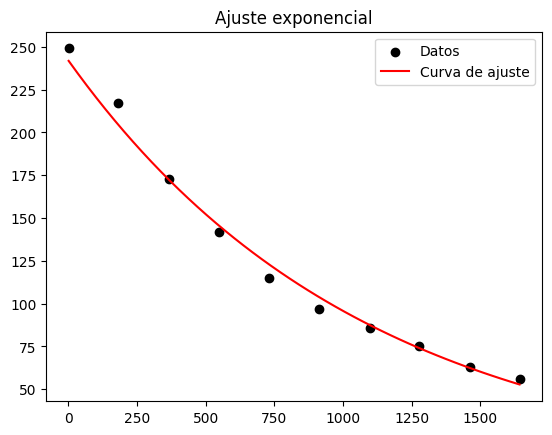
\includegraphics[width=0.82\textwidth]{imagenes/ajuste_exponencial.png}
\caption{Ajuste exponencial obtenido mediante mínimos cuadrados.}
\label{fig:ajuste}
\end{figure}

\subsection{Punto 1: Fecha estimada de cierre}

Utilizando el modelo obtenido se determinó el instante en el cual la producción diaria alcanza el valor de cierre establecido.

Se obtuvo un tiempo de:

\[
t=6176\ \text{días}
\]

Tomando como fecha inicial el 1 de enero de 2018, la fecha estimada de cierre corresponde al:

\[
\boxed{\text{28 de noviembre de 2034}}
\]

\subsection{Punto 2: Producción acumulada}

A partir de la integración del modelo exponencial se calcularon los volúmenes de producción acumulada.

Los resultados obtenidos fueron:

\begin{itemize}
    \item Producción total estimada: \textbf{394930.73 m$^3$}
    \item Producción extraída: \textbf{270555.65 m$^3$}
    \item Producción remanente: \textbf{124375.08 m$^3$}
\end{itemize}

Esto representa:

\begin{itemize}
    \item Producción extraída: \textbf{68.51\%}
    \item Producción remanente: \textbf{31.49\%}
\end{itemize}

La Figura \ref{fig:torta} muestra la distribución porcentual entre la producción extraída y la producción remanente.

\begin{figure}[H]
\centering
% If the image file is missing, show a framed placeholder instead of failing
\IfFileExists{imagenes/produccion_acumulada.png}{%
    \includegraphics[width=0.55\textwidth]{imagenes/produccion_acumulada.png}%
}{%
    \fbox{\parbox[b][0.28\textheight][c]{0.55\textwidth}{\centering Imagen ``produccion_acumulada.png'' no disponible.}}%
}
\caption{Distribución de la producción acumulada.}
\label{fig:torta}
\end{figure}

\subsection{Punto 3: Producción acumulada del 50\%}

Se determinó el instante en el cual la producción acumulada alcanza el 50\% de la producción total estimada.

Los resultados obtenidos fueron:

\begin{itemize}
    \item Producción acumulada correspondiente al 50\%: \textbf{197465.37 m$^3$}
    \item Tiempo: \textbf{992.28 días}
    \item Fecha: \textbf{18 de septiembre de 2020}
\end{itemize}

\subsection{Punto 4: Valor económico de la producción remanente}

El notebook calcula el valor económico de la producción remanente considerando:

\begin{itemize}
    \item Conversión de m$^3$ a barriles mediante el factor 6.28981.
    \item Precio del petróleo de \textbf{US\$62 por barril}.
\end{itemize}

Con estos datos se obtuvo el valor económico de la producción remanente desde el 2 de julio de 2022 hasta la fecha estimada de cierre.

\subsection{Punto 5: Producción anual}

Finalmente, se calculó el valor económico anual de la producción desde el año 2022 hasta el cierre del yacimiento.

La Figura \ref{fig:barras} presenta la evolución anual obtenida.

\begin{figure}[H]
\centering
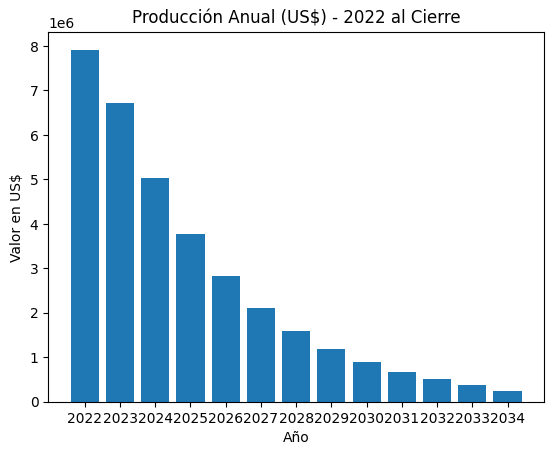
\includegraphics[width=\textwidth]{imagenes/produccion_anual.png}
\caption{Valor anual de la producción desde 2022 hasta la fecha estimada de cierre.}
\label{fig:barras}
\end{figure}

Como puede observarse, el valor económico anual disminuye progresivamente con el paso de los años, comportamiento consistente con el modelo exponencial ajustado para la producción del yacimiento. % Se agrega el contenido del archivo resultados.tex (debe estar en la misma carpeta del documento maestro)

%----------------------------------------------------------------------------------------
% Contenido del Informe - Discusión (Completar archivo discusion.tex)
%----------------------------------------------------------------------------------------
%----------------------------------------------------------------------------------------
% Contenido del Informe - Discusión
%----------------------------------------------------------------------------------------

\chapter*{Discusión}
\addcontentsline{toc}{chapter}{Discusión}

El método de ajuste por mínimos cuadrados permitió obtener una función
exponencial que representa la tendencia de los datos experimentales mediante
la minimización de la suma de los cuadrados de los errores entre los valores
medidos y los valores estimados por el modelo.

Debido a que el modelo planteado posee la forma

\[
Q(t)=Ae^{Bt},
\]

fue necesario realizar una transformación logarítmica para convertir la
expresión en un modelo lineal:

\[
\ln(Q)=\ln(A)+Bt.
\]

Esta transformación permitió aplicar el método de mínimos cuadrados lineales
para determinar los coeficientes del modelo. Una vez obtenidos dichos
coeficientes, se recuperó el valor de \(A\) aplicando la función exponencial.

El criterio utilizado por el método consiste en minimizar la suma de los
cuadrados de las diferencias entre los valores observados y los valores
estimados. Al elevar los errores al cuadrado se evita que los errores
positivos y negativos se compensen entre sí y, además, se otorga un mayor
peso a aquellas observaciones que presentan desviaciones más importantes.

La calidad del ajuste puede evaluarse mediante el error cuadrático medio
(ECM), el cual proporciona una medida global de la diferencia entre los datos
experimentales y la función obtenida. Un valor reducido del ECM indica que el
modelo reproduce adecuadamente la tendencia observada en los datos.

En este trabajo, el ajuste exponencial permitió representar el comportamiento
general de la producción del pozo y obtener una función continua a partir de
un conjunto discreto de mediciones. Esto hizo posible realizar estimaciones
para tiempos distintos de los observados experimentalmente y calcular tanto
la fecha estimada de cierre como la producción acumulada y el valor económico
remanente.

Por lo tanto, el método de mínimos cuadrados constituye una herramienta de
gran utilidad para el ajuste de datos experimentales, ya que permite obtener
una función matemática que aproxima el comportamiento real del fenómeno
estudiado y facilita la realización de análisis y predicciones posteriores.
\ % Se agrega el contenido del archivo discusion.tex (debe estar en la misma carpeta del documento maestro)

%----------------------------------------------------------------------------------------
%	CONTENIDO DE LA GUIA - APÉNDICES
%----------------------------------------------------------------------------------------

\appendix % Le indica a LaTeX que los siguientes "capítulos" son apéndices
\renewcommand{\thechapter}{\Alph{chapter}}
\renewcommand{\thesection}{\Alph{chapter}.\arabic{section}}
% Incluir los apéndices como archivos separados
% Descomentar y/o agregar las líneas para incluir nuevos apéndices

%----------------------------------------------------------------------------------------
% Contenido del Informe - Apéndice A (Completar archivo apendice_A.tex)
%----------------------------------------------------------------------------------------
%----------------------------------------------------------------------------------------
%	CONTENIDO DEL APENDICE A
%----------------------------------------------------------------------------------------

\chapter*{Apéndices}
\addcontentsline{toc}{chapter}{Apéndices} %Sirve como introducción a apéndices (no colocar este comando en los demás apéndices)

%----------------------------------------------------------------------------------------
%	LISTA DE URL DE LIKS COMPARTIDOS DE NOTEBOOKS USADAS - Colocar los Colab usados por cada alumno
%----------------------------------------------------------------------------------------
% En este bloque de líneas, escribir únicamente el link de su Colab en la última llave de las líneas newcommand
% No editar ninuan otra cosa del bloque
% Si un link posee un símbolo de porcentaje (%), anteponerle a cada % una barra invertida (\)

\ifx \AlumnoPrimero \undefined {}
\else
\newcommand{\URLColabAlumnoPrimero}{https://colab.research.google.com/drive/1-Ikn_xPvEDBBK_0eOnWAW5Hj8gZwkCO7?usp=sharing}
\fi
\ifx \AlumnoSegundo \undefined {}
\else
\newcommand{\URLColabAlumnoSegundo}{https://colab.research.google.com/drive/1-Ikn_xPvEDBBK_0eOnWAW5Hj8gZwkCO7?usp=sharing}
\fi
\ifx \AlumnoTercero \undefined {}
\else
\newcommand{\URLColabAlumnoTercero}{https://colab.research.google.com/drive/1-Ikn_xPvEDBBK_0eOnWAW5Hj8gZwkCO7?usp=sharing}
\fi
\ifx \AlumnoCuarto \undefined {}
\else
\newcommand{\URLColabAlumnoCuarto}{https://colab.research.google.com/drive/1-Ikn_xPvEDBBK_0eOnWAW5Hj8gZwkCO7?usp=sharing}
\fi
\ifx \AlumnoQuinto \undefined {}
\else
\newcommand{\URLColabAlumnoQuinto}{}
\fi
\ifx \AlumnoSexto \undefined {}
\else
\newcommand{\URLColabAlumnoSexto}{}
\fi
\ifx \AlumnoSeptimo \undefined {}
\else
\newcommand{\URLColabAlumnoSeptimo}{}
\fi
\ifx \AlumnoOctavo \undefined {}
\else
\newcommand{\URLColabAlumnoOctavo}{}
\fi

% NO EDITAR LAS SIGUIENTES LÍNEAS

\section{Notebooks de Colab} \label{sec:Colab}

A continuación, se enumeran las notebooks donde se desarrollaron los códigos mencionados en este documento:
\begin{itemize}
	\ifx \AlumnoPrimero \undefined {}
	\else
	\item \href{\URLColabAlumnoPrimero}{\underline{Notebook de \AlumnoPrimero}}
	\fi
	\ifx \AlumnoSegundo \undefined {}
	\else
	\item \href{\URLColabAlumnoSegundo}{\underline{Notebook de \AlumnoSegundo}}
	\fi
	\ifx \AlumnoTercero \undefined {}
	\else
	\item \href{\URLColabAlumnoTercero}{\underline{Notebook de \AlumnoTercero}}
	\fi
	\ifx \AlumnoCuarto \undefined {}
	\else
	\item \href{\URLColabAlumnoCuarto}{\underline{Notebook de \AlumnoCuarto}}
	\fi
	\ifx \AlumnoQuinto \undefined {}
	\else
	\item \href{\URLColabAlumnoQuinto}{\underline{Notebook de \AlumnoQuinto}}
	\fi
	\ifx \AlumnoSexto \undefined {}
	\else
	\item \href{\URLColabAlumnoSexto}{\underline{Notebook de \AlumnoSexto}}
	\fi
	\ifx \AlumnoSeptimo \undefined {}
	\else
	\item \href{\URLColabAlumnoSeptimo}{\underline{Notebook de \AlumnoSeptimo}}
	\fi
	\ifx \AlumnoOctavo \undefined {}
	\else
	\item \href{\URLColabAlumnoOctavo}{\underline{Notebook de \AlumnoOctavo}}
	\fi
\end{itemize}

 % Se agrega el contenido del archivo apendice_A.tex (debe estar en la misma carpeta del documento maestro)

\endgroup
%----------------------------------------------------------------------------------------
% Contenido del Informe - Discusión (Completar archivo referencias.bib) 
%----------------------------------------------------------------------------------------
\printbibliography[heading=bibintoc,title={Bibliografía}]  % heading=bibintoc indica incluir en índice; title define cómo se nombra a la sección
\nocite{*} % nocite indica incluir en bibliografia referencias no citadas en el cuerpo del texto


\end{document}